\documentclass{standalone}
\usepackage{tikz}
\begin{document}
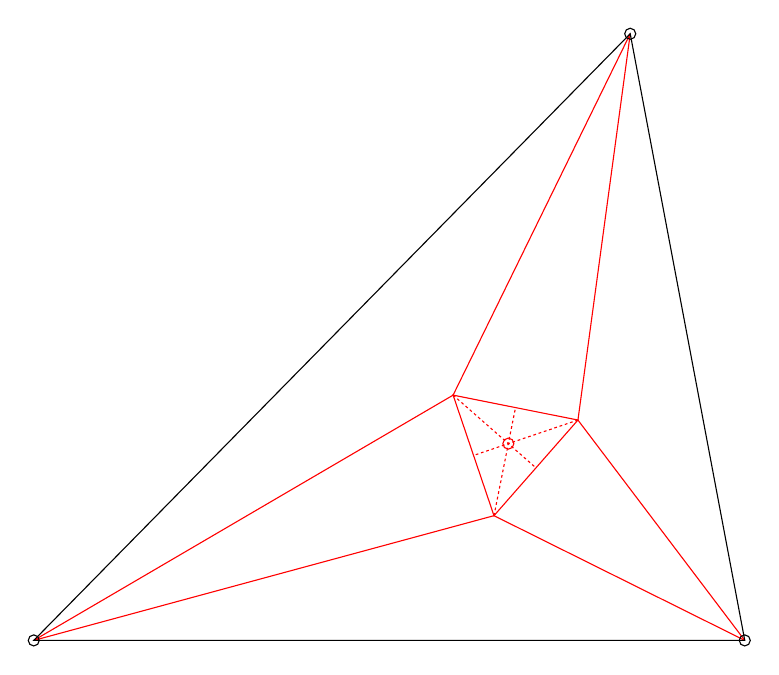
\begin{tikzpicture}[x=1pt,y=1pt]
\draw[red] (180.98,-197.56) -- (211.32,-163.00) -- (166.21,-154.00) -- cycle;
\draw[red] (14.68,-242.63) -- (180.97,-197.56);
\draw[red] (271.60,-242.63) -- (180.98,-197.56);
\draw[red] (271.60,-242.63) -- (211.31,-163.00);
\draw[red] (230.22,-23.41) -- (211.32,-163.00);
\draw[red] (230.22,-23.41) -- (166.21,-154.00);
\draw[red] (166.21,-154.00) -- (14.68,-242.63);
\draw[red, dash pattern=on 1pt] (180.98,-197.56) -- (188.76,-158.50);
\draw[red, dash pattern=on 1pt] (211.31,-163.00) -- (173.59,-175.79);
\draw[red, dash pattern=on 1pt] (166.21,-154.00) -- (196.15,-180.28);
\draw (230.21,-23.42) -- (14.68,-242.63) -- (271.60,-242.63) -- cycle;
\draw (271.60,-242.63) circle (2.00);
\draw[red] (186.17,-171.52) circle (2.00);
\draw (14.68,-242.63) circle (2.00);
\draw (230.21,-23.42) circle (2.00);
\end{tikzpicture}
\end{document}
